% Definición
\documentclass[12pt]{beamer}

% Paquetes
\usepackage{graphicx,listings}
\usepackage[utf8]{inputenc}
\usepackage[spanish,es-tabla]{babel}
\usepackage{times}          % Usar tipo Times-Roman
\usepackage[T1]{fontenc}    % Usar la codificación T1

% Datos
\title{Metodología Running Lean aplicada a un lector de noticias inteligente}
\author{Andrés M. Jiménez Ríos}
\institute[TFM]{Trabajo Fin de Máster}

% Temas
\usetheme{Boadilla}
\usecolortheme{crane}
\useoutertheme{infolines}
\useinnertheme{rectangles}

% Opciones
\setbeamertemplate{navigation symbols}{}

\lstset{
	literate={á}{{\'o}}1
	{é}{{\'e}}1
	{í}{{\'i}}1
	{ó}{{\'o}}1
	{ú}{{\'u}}1
}


\AtBeginSection{ 
	\begin{frame}{Índice} 
		\tableofcontents[currentsection]
	\end{frame}
}

\AtEndDocument{
	\frame{\titlepage}
}

% Inicio
\begin{document}

% Diapositivas
	\frame{\titlepage}
	
	\begin{frame}{Índice}
		\tableofcontents
	\end{frame}

	\section{Introducción}	
		\begin{frame}{\textit{Running Lean}}
			\begin{block}{}
				\textit{Running Lean is a systematic process for iterating from Plan A to a plan that works, before running out of resources.}
			\end{block}
			\begin{block}{Influencia}
				\begin{itemize}
                    \item Steve Blank - \textit{Customer Development}
                    \item Eric Ries - \textit{Lean Startup}
                    \item Alex Osterwalder - \textit{Bussiness Model Canvas}
                \end{itemize}
			\end{block}
        \end{frame}

        {
            \usebackgroundtemplate{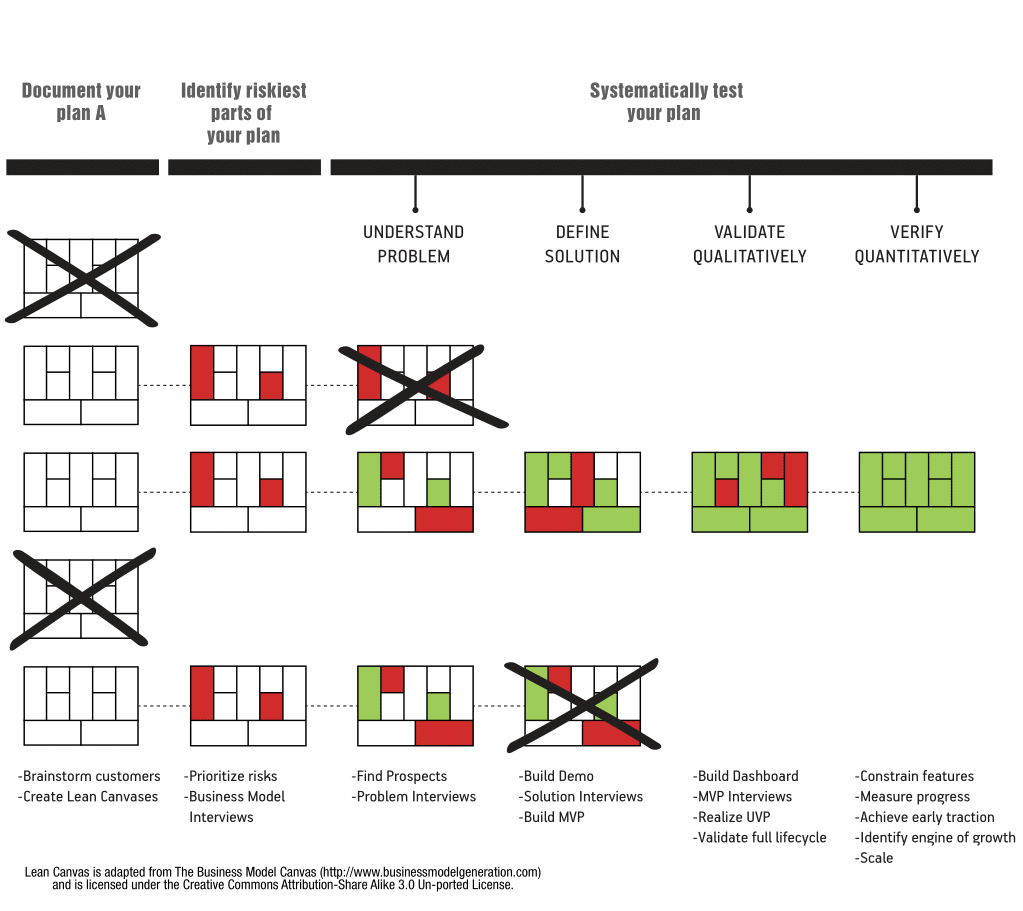
\includegraphics[height=\paperheight,width=\paperwidth]{img/lean/running_lean}}
            \setbeamertemplate{navigation symbols}{}
            \begin{frame}[plain]
            \end{frame}
        }
	
		\begin{frame}{Periodismo}
			\begin{block}{Situación actual}
				La falta de contenido de calidad, las redes sociales y las \textit{fake news}.
			\end{block}
			\begin{block}{Mundo digital}
				Su propuestas son la sindicación de contenido, las redes sociales y aplicaciones propias.
			\end{block}
		\end{frame}
\end{document}